\documentclass[10pt,a4paper]{report}

\usepackage{geometry}
\usepackage{todo}   
\usepackage{amssymb}
\usepackage{graphicx} 
\usepackage{pifont}
         % graphiques de base
% Include figure files
%\usepackage{dcolumn}% Align table columns on decimal point
\usepackage{amsmath,amsfonts}%
\usepackage{amsthm}
\usepackage{xcolor}
\usepackage{bm}%
\usepackage{psfrag}%
\usepackage{pict2e}
\usepackage{mdframed,verbatim}
\usepackage[tikz]{bclogo}
\usepackage{epstopdf}
\usepackage{algpseudocode}
\usepackage{algorithm}
\usepackage[colorlinks=true, pdfstartview=FitV, linkcolor=blue, 
            citecolor=blue, urlcolor=blue]{hyperref}
\usepackage{tikz}
\usetikzlibrary{calc,patterns,decorations.pathmorphing,decorations.markings}

\usepackage{tabularx}
\usepackage{cancel}
     \usepackage{aliascnt}
\usepackage[capitalise]{cleveref}
\usepackage[inline]{showlabels}



\newif\ifsolutions
\solutionstrue 
%\solutionsfalse 

\usepackage{commands_od}
	
\usepackage{array}

\title{\Large \textbf{Refresher courses in Mathematics}\\\
}

\author{Olivier DAZEL \& Mathieu GABORIT}



% ------------------- Title and Author -----------------------------

\begin{document}

\maketitle




\chapter{Matrices}


\section{Algebraic Calculus}

\input{../TeX_Files/Matrices/Algebraic_Calculus_1}
\input{../TeX_Files/Matrices/Algebraic_Calculus_2}
\input{../TeX_Files/Matrices/Algebraic_Calculus_3}
\input{../TeX_Files/Matrices/Algebraic_Calculus_4}
\bexo
Let consider the following matrix
\begin{equation}
	\mat{M}=\begin{bmatrix}
		0&1&0&0&0\\
		0&0&1&0&0\\
		0&0&0&1&0\\
		0&0&0&0&1\\
		1&0&0&0&0
	\end{bmatrix}
\end{equation}
\begin{itemize}
	\item What is the value of $\det{\mat{M}}$ ?
	\item What is the value of $\mat{M}^5$ ?
	\item What is the value of $\det{\mat{M}}$ ? 
\end{itemize}


\eexo 

\solution{}
	





\bexo
The rotation matrices $[\tb{R}_x(\theta_x)]$, $[\tb{R}_y(\theta_y)]$ and $[\tb{R}_z(\theta_z)]$
are respectively defined by:
\begin{equation}
	[\tb{R}_x(\theta_x)]=\begin{bmatrix}
		1&0&0\\
		0 & \cos(\theta_x) &\sin(\theta_x)\\
		0 & -\sin(\theta_x) &\cos(\theta_x) 
	\end{bmatrix}\esp 
	[\tb{R}_y(\theta_y)]=\begin{bmatrix}
	\cos(\theta_y) &0&\sin(\theta_y)\\
0&1&0\\
-\sin(\theta_y)&0&\cos(\theta_y) 
	\end{bmatrix}
	\esp 
\end{equation}
\begin{equation}
[\tb{R}_z(\theta_z)]=\begin{bmatrix}
		\cos(\theta_z) &\sin(\theta_z)&0\\
		-\sin(\theta_z) &\cos(\theta_z)& 0\\
		0&0&1 
	\end{bmatrix}
\end{equation}

\begin{itemize}
	\item What is the determinant of $[\tb{R}_x(\theta_x)][\tb{R}_y(\theta_y)][\tb{R}_z(\theta_z)]$ ?
	\item What is the value of $[\tb{R}_x(\pi/2)][\tb{R}_y(\pi/2)][\tb{R}_z(\pi/2)]$ and the value of $[\tb{R}_z(\pi/2)][\tb{R}_y(\pi/2)][\tb{R}_x(\pi/2)]$ ? Comment this result.
\end{itemize}


Compute the following transformations:
 




\eexo 

\solution{}
	





\bexo
The Hooke's matrix $\mat{C}$ for 
a material relates the vector of strain $\bs{\eps}$ to the vector of stresses $\bs{\sigma}$. 
\begin{equation}
	\bs{\sigma}=\mat{C}\bs{\eps}.
\end{equation}
For an isotropic material, the Hooke's matrix depends on only two coefficients called the Lamé coeeficients $\lambda$ and $\mu$ and
\begin{equation}
	\mat{C}=
	\begin{bmatrix}
		\lambda+2\mu & \lambda & \lambda &0&0&0\\
		 \lambda &\lambda+2\mu & \lambda &0&0&0\\
		 \lambda &\lambda &\lambda+2\mu & 0&0&0\\
		 0&0&0&\mu &0&0\\
		 0&0&0&0&\mu &0\\
		 0&0&0&0&0&\mu  
	\end{bmatrix}
\end{equation}
The compliance matrix $\mat{S}$ is defined as the inverse of $\mat{C}$. \\

What is the value of the compliance matrix ?


\eexo 

\solution{}
	





%\input{../TeX_Files/Matrices/Algebraic_Calculus}


\section{Determinant of matrices}
\bexo
What is the determinant of 
\begin{equation}
\mat{M}=
\begin{bmatrix}
	1& 0& 0& 0\\
0& 1& 0& 1\\
1& 0& 1& 1\\
2& 3& 1& 1
\end{bmatrix}?
\end{equation}

\eexo
\solution{
The expansion along the first row leads to 
\begin{equation}
	\det{\mat{M}}=1\times \begin{vmatrix}
		1& 0& 1\\
0& 1& 1\\
 3& 1& 1
	\end{vmatrix}=-3
\end{equation}

}

\bexo
What is the link between determinants of matrice $\mat{M}$ and $\mat{N}$ defined by 
\begin{equation}
\mat{M}=
\begin{bmatrix}
	1& 0& 0& 0\\
0& 1& 0& 1\\
1& 0& 1& 1\\
2& 3& 1& 1
\end{bmatrix} \esp
\mat{N}=
\begin{bmatrix}
	1& 0& 0& 0\\
0& 1& 0& 5\\
1& 0& 1& 5\\
2& 3& 1& 5
\end{bmatrix}
\end{equation}
\eexo

\solution{The two matrices are identical except in the last column. The column of $\mat{N}$ is 5 times the column of $\mat{M}$ then the determinant of $\mat{N}$ is 5 times the determinant of $\mat{M}$}


\bexo
What is the determinant of 
\begin{equation}
\mat{M}=
\begin{bmatrix}
	1& 2& 0& 0\\
2& 1& 0& 0\\
0& 0& 1& 1\\
0& 0& 1& -1
\end{bmatrix} ?
\end{equation}
\eexo

\solution{
\begin{equation}
	\det{\mat{M}}=\begin{vmatrix}
1 & 2\\ 2 & 1	
\end{vmatrix}\times
\begin{vmatrix}
1 & 1\\ 1 & -1	
\end{vmatrix}=(-3)\times(-2)=6
\end{equation}
}


\bexo
What is the determinant of 
\begin{equation}
\mat{M}=
\begin{bmatrix}
	1& 1& 1\\
1& 2& 3\\
1& 4& 9
\end{bmatrix} ?
\end{equation}
\eexo

\solution{
\begin{equation}
	\det{\mat{M}}=(2-1)(3-1)(3-2)=2
\end{equation}
}


\bexo
What is the determinant of 
\begin{equation}
\mat{M}=
\begin{bmatrix}
	2& -1& 0\\
-1& 2& -1\\
0& -1& 2
\end{bmatrix} ?
\end{equation}
\eexo

\solution{
\begin{equation}
	\det{\mat{M}}=2
	\begin{vmatrix}
		2 & -1\\-1 & 2
	\end{vmatrix}-(-1)
		\begin{vmatrix}
		-1 & -1\\0 & 2
	\end{vmatrix}=6-2=4
\end{equation}
}


\bexo
What is the determinant of 
\begin{equation}
\mat{M}=
\begin{bmatrix}
	1& -1& 0\\
-1& 2& -1\\
0& -1& 1
\end{bmatrix} ?
\end{equation}
\eexo

\solution{
The sum of the three lines is zero. They are then linearly dependent. The determinant is zero}


\bexo
Given

\begin{equation}
	\mat{A} = \begin{bmatrix}
		1& 1& 0& 3\\
		3& 4& 1& 3\\
		1& 1& 0& 1\\
		1& 0& 0& 3
	\end{bmatrix}
	~~,~~
	\mat{P} = \begin{bmatrix}
		1& 0& 0& 0\\
		0& 0& 0& 1\\
		0& 0& 1& 0\\
		0& 1& 0& 0
	\end{bmatrix}
\end{equation}

evaluate:

\begin{enumerate}
	\item $\mat{P}\mat{A}$
	\item $\mathrm{det}(\mat{A})$
	\item $\mathrm{det}(\mat{P}\mat{A})$
\end{enumerate}

What is the effect of $\mat{P}$ on $\mat{A}$?
\eexo

\solution{

\hfill\\
\begin{enumerate}
	\item $$\mat{P}\mat{A} = \begin{bmatrix}
			1& 1& 0& 3\\
			1& 0& 0& 3\\
			1& 1& 0& 1\\
			3& 4& 1& 3
		\end{bmatrix}$$
	\item $2$
	\item $-2$
\end{enumerate}

$\mat{P}$ \textit{permutes} 2 lignes of $\mat{A}$.
}


\bexo
Given

\begin{equation}
	\mat{A} = \begin{bmatrix}
		1& 0& 0& 0\\
		0& 1& 0& 1\\
		1& 0& 1& 1\\
		2& 3& 1& 1
	\end{bmatrix}
	~~,~~
	\mat{P}_1 = \begin{bmatrix}
		0& 0& 1& 0\\
		0& 0& 0& 1\\
		1& 0& 0& 0\\
		0& 1& 0& 0
	\end{bmatrix}
	~~,~~
	\mat{P}_2 = \begin{bmatrix}
		1& 0& 0& 0\\
		0& 0& 0& 1\\
		0& 0& 1& 0\\
		0& 1& 0& 0
	\end{bmatrix}
\end{equation}

evaluate:

\begin{enumerate}
	\item $\mathrm{det}(\mat{A})$
	\item $\mathrm{det}(\mat{P}_1\mat{A})$
	\item $\mathrm{det}(\mat{P}_2\mat{A})$
\end{enumerate}

Can you deduce a more general rule for the determinants of permutated matrices?
\eexo

\solution{
\hfill\\
\begin{enumerate}
	\item $-3$
	\item $-3$
	\item $3$
\end{enumerate}

The permutation matrix has a determinant of $(-1)^N$ with $N$ the number of permutations.
}


\bexo
Given
\begin{equation}
	A = \begin{bmatrix}
		1& 0\\ 1& 2
	\end{bmatrix}
	~~,~~
	B = \begin{bmatrix}
		7& 9\\ 0& 2
	\end{bmatrix}
	~~,~~
	C = \begin{bmatrix}
		5& 6\\ 4& 3
	\end{bmatrix}
	~~,~~
	D = \begin{bmatrix}
		2& 4\\ 5& 6
	\end{bmatrix}
\end{equation}

and $\mathbf{0}_n$ a $n\times n$ matrix of zeros;

evaluate

\begin{equation}
\det{\begin{matrix}
	\mat{A}& \mathbf{0}_2\\
	\mathbf{0}_2 & \mat{D}\\
\end{matrix}}
~~,~~
\det{\begin{matrix}
	\mat{A}& \mat{B}\\
	\mathbf{0}_2 & \mat{D}\\
\end{matrix}}
~~,~~
\det{\begin{matrix}
	\mat{A}& \mathbf{0}_2\\
	\mat{C} & \mat{D}\\
\end{matrix}}
\end{equation}

What rule(s) can you deduce from the previous calculations?
\eexo


\solution{
	The three matrices have the same determinant ($-16$), the extra-diagonal \textit{block} does not come in play.
	The following equivalence then holds:
	\begin{equation}
		\det{\begin{matrix}
			\mat{A}& \mat{B}\\
			\mathbf{0}_2 & \mat{D}\\
		\end{matrix}}
		=
		\det{\begin{matrix}
			\mat{A}& \mathbf{0}_2\\
			\mat{C} & \mat{D}\\
		\end{matrix}}
		=
		\mathrm{det}(\mat{A})
		\mathrm{det}(\mat{D})
	\end{equation}
}

%% !TEX root = ../RAN_MFA.tex

\bexo
What is the determinant of 
\begin{equation*}
\left[
\begin{array}{cc}
a & b \\
d & c
\end{array}
\right]
\end{equation*}
\eexo\solution{
\begin{equation*}
ac-bd
\end{equation*}
}

%%%%%%%%%%%%%%

\bexo
What is the determinant of 
\begin{equation*}
\left[
\begin{array}{cc}
-3 & 0 \\
-5 & 0
\end{array}
\right]
\end{equation*}

\eexo\solution{
\begin{equation*}
0
\end{equation*}
}




\bexo
What is the determinant of 
\begin{equation*}
\left[
\begin{array}{cc}
a & 34 \\
b & c
\end{array}
\right]
\end{equation*}

\eexo\solution{
\begin{equation*}
ac-34b
\end{equation*}
}




\bexo
What is the determinant of 
\begin{equation*}
\left[
\begin{array}{ccc}
x & x' & x'' \\
y & y' & y''\\
z & z' & z''
\end{array}
\right]
\end{equation*}
\eexo\solution{
\begin{equation*}
xy'z''+x'y''z+x''yz'-xy''z'-x'yz''-x''y'z
\end{equation*}
}

%%%%%%%%%%%%%%%%%%%%%%%%%%%%%%%%%%%

\bexo
What is the determinant of 
\begin{equation*}
\left[
\begin{array}{ccc}
    -4  &  -5  &   0\\
    -2  &   5  &  -6\\
    -5  &   5  &  -4
\end{array}
\right]
\end{equation*}

\eexo\solution{
\begin{equation*}
-150
\end{equation*}
}


\bexo
What is the determinant of 
\begin{equation*}
\left[
\begin{array}{ccc}
    -2 &   -6  &   2\\
     3 &   -4  &   1\\
    -6 &    1  &  -1
\end{array}
\right]
\end{equation*}

\eexo\solution{
\begin{equation*}
-30
\end{equation*}
}

\bexo
What is the determinant of 
\begin{equation*}
\left[
\begin{array}{cccc}
     6  &   6  &   7 &   -6\\
     5  &   0  &   1 &   -4\\
     2  &  -3  &   2 &   -1\\
    -3  &   8  &   1 &   -6
\end{array}
\right]
\end{equation*}

\eexo\solution{
\begin{equation*}
918
\end{equation*}
}
%%%%%%%%%%%%%%%%%%%%%%%%%%%%%

%$X, Y, X'$ are vectors. $a,b\in \mathbb{R}$. What is the determinant of 
%\[aX+bY,X'\]
%\eexo\solution{
%\begin{equation*}
%a\det{X,X'}+b\det{Y,X'}
%\end{equation*}
%}
%\autre{
%\begin{equation*}
%(a+b)\left(\det{X,X'}+\det{Y,X'}\right)
%\end{equation*}
%}
%\autre{
%\begin{equation*}
%b\det{X,X'}+a\det{Y,X'}
%\end{equation*}
%}
%%%%%%%%%%%%%%%%%%%%%%%%%%%%%%%%%%%
\bexo
What is the determinant of 
\[
\left[
\begin{array}{cc}
7 & 11\\
-8 & 4
\end{array}
\right]
\]
\eexo\solution{
\begin{equation*}
116
\end{equation*}
}

%%%%%%%%%%%%%%%%%%%%%%%%%%%%%%%%%%%
\bexo
What is the determinant of 
\[
\left[
\begin{array}{cccc}
a_{11} & a_{12} & a_{13} & a_{14}\\
0 & a_{22} & a_{23} & a_{24}\\
0 & 0 & a_{33} & a_{34}\\
0 & 0 & 0 & a_{44}\\
\end{array}
\right]
\]
\eexo\solution{
\begin{equation*}
a_{11}a_{22}a_{33}a_{44}
\end{equation*}
}

%%%%%%%%%%%%%%%%%%%%%%%%%%%%%%%%%%%
\bexo
What is the determinant of 
\[
\left[
\begin{array}{ccc}
1 & 0 & 6\\
3 & 4 & 15\\
5 & 6 & 21
\end{array}
\right]
\]
\eexo\solution{
\begin{equation*}
-18
\end{equation*}
}

%%%%%%%%%%%%%%%%%%%%%%%%%%%%%%%%%%%
\bexo
What is the determinant of 
\[
\left[
\begin{array}{ccc}
1& 0 &2\\
3 &4 &5\\
5 &6& 7\end{array}
\right]
\]
\eexo\solution{
\begin{equation*}
-6
\end{equation*}
}

%%%%%%%%%%%%%%%%%%%%%%%%%%%%%%%%%%%
\bexo
What is the determinant of 
\[
\left[
\begin{array}{ccc}
1 &0 &-1\\
2&3&5\\
4&1&3\end{array}
\right]
\]
\eexo\solution{
\begin{equation*}
14
\end{equation*}
}

%%%%%%%%%%%%%%%%%%%%%%%%%%%%%%%%%%%
\bexo
What is the determinant of 
\[
\left[
\begin{array}{cccc}
0& 1& 2& 3\\
1 &2& 3& 0\\
2 &3& 0& 1\\
3 &0& 1& 2
\end{array}
\right]
\]
\eexo\solution{
\begin{equation*}
96
\end{equation*}
}

%%%%%%%%%%%%%%%%%%%%%%%%%%%%%%%%%%%
\bexo
What is the determinant of 
\[
\left[
\begin{array}{cccc}
0& 1& 1 &0\\
1& 0& 0 &1\\
1& 1& 0 &1\\
1& 1& 1 &0
\end{array}
\right]
\]
\eexo\solution{
\begin{equation*}
-1
\end{equation*}
}

%%%%%%%%%%%%%%%%%%%%%%%%%%%%%%%%%%%
\bexo
What is the determinant of 
\[
\left[
\begin{array}{cccc}
1& 2& 1& 2\\
1& 3& 1& 3\\
2& 1& 0& 6\\
1& 1& 1& 7
\end{array}
\right]
\]
\eexo\solution{
\begin{equation*}
-12
\end{equation*}
}

%%%%%%%%%%%%%%%%%%%%%%%%%%%%%%%%%%%
\bexo
What is the determinant of 
\[
\left[
\begin{array}{ccc}
a& b& c\\
c& a& b\\
b& c& a
\end{array}
\right]
\]
\eexo\solution{
\begin{equation*}
a^3+b^3+c^3-3abc
\end{equation*}
}

%%%%%%%%%%%%%%%%%%%%%%%%%%%%%%%%%%%
\bexo
What is the determinant of 
\[
\left[
\begin{array}{cccc}
1& 0& 0& 1\\
0& 1& 0& 0\\
1& 0& 1& 1\\
2& 3& 1& 1
\end{array}
\right]
\]
\eexo\solution{
\begin{equation*}
-1
\end{equation*}
}

%%%%%%%%%%%%%%%%%%%%%%%%%%%%%%%%%%%
\bexo
What is the determinant of 
\[
\left[
\begin{array}{cccc}
-1& 1& 1& 1\\
1& -1& 1& 1\\
1& 1& -1& 1\\
1& 1& 1& -1\end{array}
\right]
\]
\eexo\solution{
\begin{equation*}
-16
\end{equation*}
}

%%%%%%%%%%%%%%%%%%%%%%%%%%%%%%%%%%%
\bexo
What is the determinant of 
\[
\left[
\begin{array}{cccc}
10& 0& -5& 15\\
-2& 7& 3& 0\\
8& 14& 0& 2\\
0& -21& 1& -1\end{array}
\right]
\]
\eexo\solution{
\begin{equation*}
7840
\end{equation*}
}

%%%%%%%%%%%%%%%%%%%%%%%%%%%%%%%%%%%
\bexo
What is the determinant of 
\[
\left[
\begin{array}{cccc}
a& a& b& 0\\
a& a& 0& b\\
c& 0& a& a\\
0& c& a& a
\end{array}
\right]
\]
\eexo\solution{
\begin{equation*}
bc(bc-4a^2)
\end{equation*}
}

%%%%%%%%%%%%%%%%%%%%%%%%%%%%%%%%%%%
\bexo
What is the determinant of 
\[
\left[
\begin{array}{ccccc}
1& 0& 3& 0& 0\\
0& 1& 0& 3& 0\\
a& 0& a& 0& 3\\
b& a& 0& a& 0\\
0& b& 0& 0& a
\end{array}
\right]
\]
\eexo\solution{
\begin{equation*}
4a^3+27b^2
\end{equation*}
}
%%%%%%%%%%%%%%%%%%%%%%%%%%%%%%%%%%%
\bexo
What is the determinant of 
\[
\left[
\begin{array}{ccccc}
1& 0& 0& 1& 0\\
0& -4& 3& 0& 0\\
-3& 0& 0& -3& -2\\
0& 1& 7& 0& 0\\
4& 0& 0& 7& 1
\end{array}
\right]
\]
\eexo\solution{
\begin{equation*}
186
\end{equation*}
}

%%%%%%%%%%%%%%%%%%%%%%%%%%%%%%%%%%%
\bexo
What is the determinant of 
\[
\left[
\begin{array}{cccc}
a_1 & a_2 & \cdots & a_n\\
a_1 & a_1 & \ddots & \vdots\\
\vdots & \ddots & \ddots & a_2\\
a_1 & \cdots & a_1 & a_1
\end{array}
\right]
\]
\eexo\solution{
\begin{equation*}
a_1(a_1-a_2)^{n-1}
\end{equation*}
}



\section{Change of basis}

% !TEX root = ../RAN_MFA.tex

\bexo
What is the image $[\tb{M}']$ of 
$[\tb{M}]=\left[
\begin{array}{cc}
2 & -1 \\
-1 & 2
\end{array}
\right]
$
 in the 
$\left[
\begin{array}{cc}
1 & 1 \\
1 & -1
\end{array}
\right]
$ basis

\eexo\solution{
\begin{equation*}
[\tb{M}']=\left[
\begin{array}{cc}
3 & 0 \\
0 & 1
\end{array}
\right]
\end{equation*}
}

\bexo
What is the image $[\tb{M}']$ of 
$[\tb{M}]=\left[
\begin{array}{cc}
1 & 1 \\
1 & -1
\end{array}
\right]
$
 in the 
$\left[
\begin{array}{cc}
\dfrac{\sqrt{2}}{2} & \dfrac{\sqrt{2}}{2} \\
\dfrac{\sqrt{2}}{2} & -\dfrac{\sqrt{2}}{2}
\end{array}
\right]
$ basis

\eexo\solution{
\begin{equation*}
[\tb{M}']=\left[
\begin{array}{cc}
1 & 1 \\
1 & -1
\end{array}
\right]
\end{equation*}
}


\bexo
What is the image $[\tb{M}']$ of 
$[\tb{M}]=\left[
\begin{array}{cc}
2 & 3 \\
1 & 2
\end{array}
\right]
$
 in the 
$\left[
\begin{array}{cc}
1 & 2 \\
0& 1
\end{array}
\right]
$ basis

\eexo\solution{
\begin{equation*}
[\tb{M}']=\left[
\begin{array}{cc}
0 & -1 \\
1 & 4
\end{array}
\right]
\end{equation*}
}

%\bexo
%What is the image $[\tb{M}']$ of 
%$[\tb{M}]=\left[
%\begin{array}{cc}
%3 & 3 \\
%1 & 5
%\end{array}
%\right]
%$
% in the 
%$\left[
%\begin{array}{cc}
%1 & 2 \\
%1& 1
%\end{array}
%\right]
%$ basis
%
%\eexo\solution{
%\begin{equation*}
%[\tb{M}']=\left[
%\begin{array}{cc}
%6 & 5 \\
%0 & 2
%\end{array}
%\right]
%\end{equation*}
%}
%
%
%\bexo
%What is the image $[\tb{M}']$ of 
%$[\tb{M}]=\left[
%\begin{array}{cc}
%5 & 10 \\
%15 & 20
%\end{array}
%\right]
%$
% in the 
%$\left[
%\begin{array}{cc}
%2 & 10 \\
%3 & 5
%\end{array}
%\right]
%$ basis
%
%\eexo\solution{
%\begin{equation*}
%[\tb{M}']=\left[
%\begin{array}{cc}
%35 & 100 \\
%-3 & -10
%\end{array}
%\right]
%\end{equation*}
%}





\section{Eigenvalues and Eigenvectors}

%

% !TEX root = ../RAN_MFA.tex


\bexo
What are the eigenvalues of 
\begin{equation*}
\left[
\begin{array}{cc}
1 & 2 \\
0 & 2
\end{array}
\right]
\end{equation*}
For each eigenvalue $\lambda$, propose one eigenvector $\tb{X}$
\eexo\solution{
\begin{equation*}
\lambda=1 \esp \tb{X}=\left\{
\begin{array}{c}
1\\
0
\end{array}
\right\}
\end{equation*}
\begin{equation*}
\lambda=2 \esp \tb{X}=\left\{
\begin{array}{c}
2\\
1
\end{array}
\right\}
\end{equation*}
}
%%%%%%%%%%%%%%%%%%%%%%%%%%%%%%%%%%
\bexo
What are the eigenvalues of 
\begin{equation*}
\left[
\begin{array}{cc}
2 & -1 \\
-1 & 2
\end{array}
\right]
\end{equation*}
For each eigenvalue $\lambda$, propose one eigenvector $\tb{X}$
\eexo\solution{
\begin{equation*}
\lambda=1 \esp \tb{X}=\left\{
\begin{array}{c}
1\\
1
\end{array}
\right\}
\end{equation*}
\begin{equation*}
\lambda=3 \esp \tb{X}=\left\{
\begin{array}{c}
1\\
-1
\end{array}
\right\}
\end{equation*}
}
%%%%%%%%%%%%%%%%%%%%%%%%%%%%%%%%%%%%%%%%%%%%%%%%%
%\bexo
%What are the eigenvalues of 
%\begin{equation*}
%\left[
%\begin{array}{cc}
%3 & 2 \\
%1 & 2
%\end{array}
%\right]
%\end{equation*}
%For each eigenvalue $\lambda$, propose one eigenvector $\tb{X}$
%\eexo\solution{
%\begin{equation*}
%\lambda=1 \esp \tb{X}=\left\{
%\begin{array}{c}
%-1\\
%1
%\end{array}
%\right\}
%\end{equation*}
%\begin{equation*}
%\lambda=4 \esp \tb{X}=\left\{
%\begin{array}{c}
%2\\
%1
%\end{array}
%\right\}
%\end{equation*}
%}
%%%%%%%%%%%%%%%%%%%%%%%%%%%%%%%%%%%%%%%%%%%%%%%%%%
%
%\bexo
%What are the eigenvalues of 
%\begin{equation*}
%\left[
%\begin{array}{cc}
%1 & 2 \\
%3 & 4
%\end{array}
%\right]
%\end{equation*}
%For each eigenvalue $\lambda$, propose one eigenvector $\tb{X}$
%\eexo\solution{
%\begin{equation*}
%\lambda=\frac{5+\sqrt{33}}{2} \esp \tb{X}=\left\{
%\begin{array}{c}
%1\\
%\frac{3+\sqrt{33}}{2}
%\end{array}
%\right\}
%\end{equation*}
%\begin{equation*}
%\lambda=\frac{5-\sqrt{33}}{2} \esp \tb{X}=\left\{
%\begin{array}{c}
%1\\
%\frac{3-\sqrt{33}}{2}
%\end{array}
%\right\}
%\end{equation*}
%}
%%%%%%%%%%%%%%%%%%%%%%%%%%%%%%%%%%%%%%%%%%%%%%%%%%
%
%\bexo
%What are the eigenvalues of 
%\begin{equation*}
%\left[
%\begin{array}{cc}
%1 & 2 \\
%3 & 4
%\end{array}
%\right]
%\end{equation*}
%For each eigenvalue $\lambda$, propose one eigenvector $\tb{X}$
%\eexo\solution{
%\begin{equation*}
%\lambda=8+\sqrt{5} \esp \tb{X}=\left\{
%\begin{array}{c}
%1\\
%\frac{7+\sqrt{5}}{4}
%\end{array}
%\right\}
%\end{equation*}
%\begin{equation*}
%\lambda=8-\sqrt{5} \esp \tb{X}=\left\{
%\begin{array}{c}
%1\\
%\frac{7-\sqrt{5}}{4}
%\end{array}
%\right\}
%\end{equation*}
%}
%%%%%%%%%%%%%%%%%%%%%%%%%%%%%%%%%%%%%%%%%%%%%%%%%%
%
%
%\bexo
%What are the eigenvalues of 
%\begin{equation*}
%\left[
%\begin{array}{cc}
%3 & 0 \\
%2 & 1
%\end{array}
%\right]
%\end{equation*}
%For each eigenvalue $\lambda$, propose one eigenvector $\tb{X}$
%\eexo\solution{
%\begin{equation*}
%\lambda=1 \esp \tb{X}=\left\{
%\begin{array}{c}
%0\\
%1
%\end{array}
%\right\}
%\end{equation*}
%\begin{equation*}
%\lambda=3 \esp \tb{X}=\left\{
%\begin{array}{c}
%1\\
%0
%\end{array}
%\right\}
%\end{equation*}
%}
%%%%%%%%%%%%%%%%%%%%%%%%%%%%%%%%%%%%%%%%%%%%%%%%%%
%\bexo
%What are the eigenvalues of 
%\begin{equation*}
%\left[
%\begin{array}{cc}
%4 & 3 \\
%1 & 1
%\end{array}
%\right]
%\end{equation*}
%For each eigenvalue $\lambda$, propose one eigenvector $\tb{X}$
%\eexo\solution{
%\begin{equation*}
%\lambda=\frac{5+\sqrt{21}}{2} \esp \tb{X}=\left\{
%\begin{array}{c}
%\frac{3+\sqrt{21}}{2}\\
%1
%\end{array}
%\right\}
%\end{equation*}
%\begin{equation*}
%\lambda=\frac{5-\sqrt{21}}{2} \esp \tb{X}=\left\{
%\begin{array}{c}
%\frac{3-\sqrt{21}}{2}\\
%1
%\end{array}
%\right\}
%\end{equation*}
%}
%%%%%%%%%%%%%%%%%%%%%%%%%%%%%%%%%%%%%%%%%%%%%%%%%%
%
%
%\bexo
%What are the eigenvalues of 
%\begin{equation*}
%\left[
%\begin{array}{cc}
%1 & 2 \\
%2 & 1
%\end{array}
%\right]
%\end{equation*}
%For each eigenvalue $\lambda$, propose one eigenvector $\tb{X}$
%\eexo\solution{
%\begin{equation*}
%\lambda=-1 \esp \tb{X}=\left\{
%\begin{array}{c}
%-1\\
%1
%\end{array}
%\right\}
%\end{equation*}
%\begin{equation*}
%\lambda=3 \esp \tb{X}=\left\{
%\begin{array}{c}
%1\\
%1
%\end{array}
%\right\}
%\end{equation*}
%}
%%%%%%%%%%%%%%%%%%%%%%%%%%%%%%%%%%%%%%%%%%%%%%%%%%
%\bexo
%What are the eigenvalues of 
%\begin{equation*}
%\left[
%\begin{array}{cc}
%1 & 1\\
%2 & 1\\
%\end{array}
%\right]
%\end{equation*}
%For each eigenvalue $\lambda$, propose one eigenvector $\tb{X}$
%\eexo\solution{
%\begin{equation*}
%\lambda=1+\sqrt{2} \esp \tb{X}=\left\{
%\begin{array}{c}
%1\\
%\sqrt{2}
%\end{array}
%\right\}
%\end{equation*}
%\begin{equation*}
%\lambda=1-\sqrt{2} \esp \tb{X}=\left\{
%\begin{array}{c}
%1\\
%-\sqrt{2}
%\end{array}
%\right\}
%\end{equation*}
%
%}
%%%%%%%%%%%%%%%%%%%%%%%%%%%%%%%%%%%%%%%%%%%%%%%%%%%%%%%%
%
%\bexo
%What are the eigenvalues of 
%\begin{equation*}
%\left[
%\begin{array}{cc}
%3 & 1\\
%3 & 3\\
%\end{array}
%\right]
%\end{equation*}
%For each eigenvalue $\lambda$, propose one eigenvector $\tb{X}$
%\eexo\solution{
%\begin{equation*}
%\lambda=3+\sqrt{3} \esp \tb{X}=\left\{
%\begin{array}{c}
%1\\
%\sqrt{3}
%\end{array}
%\right\}
%\end{equation*}
%\begin{equation*}
%\lambda=3-\sqrt{3} \esp \tb{X}=\left\{
%\begin{array}{c}
%1\\
%-\sqrt{3}
%\end{array}
%\right\}
%\end{equation*}
%
%}
%%%%%%%%%%%%%%%%%%%%%%%%%%%%%%%%%%%%%%%%%%%%%%%%%%%%%%%%
%
%
%\bexo
%What are the eigenvalues of 
%\begin{equation*}
%\left[
%\begin{array}{ccc}
%1 & 0 & 0\\
%0 & 1 & 0\\
%1 & -1 & 2
%\end{array}
%\right]
%\end{equation*}
%For each eigenvalue $\lambda$, propose one eigenvector $\tb{X}$
%\eexo\solution{
%\begin{equation*}
%\lambda=1 \esp \tb{X}_1=\left\{
%\begin{array}{c}
%1\\
%1\\
%0
%\end{array}
%\right\}
%\esp
%\tb{X}_2=\left\{
%\begin{array}{c}
%0\\
%1\\
%1
%\end{array}
%\right\}
%\end{equation*}
%\begin{equation*}
%\lambda=2 \esp \tb{X}=\left\{
%\begin{array}{c}
%0\\
%0\\
%1
%\end{array}
%\right\}
%\end{equation*}}
%%%%%%%%%%%%%%%%%%%%%%%%%%%%%%%%%%%%%%%%%%%%%%%%%%
%
%\bexo
%What are the eigenvalues of 
%\begin{equation*}
%\left[
%\begin{array}{ccc}
%2 & -1 &0\\
%-1 & 2 &-1\\
%0 & -1 &2
%\end{array}
%\right]
%\end{equation*}
%For each eigenvalue $\lambda$, propose one eigenvector $\tb{X}$
%\eexo\solution{
%\begin{equation*}
%\lambda=2 \esp \tb{X}=\left\{
%\begin{array}{c}
%1\\
%0\\
%-1
%\end{array}
%\right\}
%\end{equation*}
%
%\begin{equation*}
%\lambda=2+\sqrt{2} \esp \tb{X}=\left\{
%\begin{array}{c}
%1\\
%-\sqrt{2}\\
%1
%\end{array}
%\right\}
%\end{equation*}
%\begin{equation*}
%\lambda=2-\sqrt{2} \esp \tb{X}=\left\{
%\begin{array}{c}
%1\\
%\sqrt{2}\\
%1
%\end{array}
%\right\}
%\end{equation*}
%}
%%%%%%%%%%%%%%%%%%%%%%%%%%%%%%%%%%%%%%%%%%%%%%%%%%%%%%%%
%
%
%\bexo
%What are the eigenvalues of 
%\begin{equation*}
%\left[
%\begin{array}{ccc}
%0 & 1 & 1\\
%1 & 0 & 1\\
%1 & 1 & 0
%\end{array}
%\right]
%\end{equation*}
%For each eigenvalue $\lambda$, propose one eigenvector $\tb{X}$
%\eexo\solution{
%\begin{equation*}
%\lambda=-1 \esp \tb{X}_1=\left\{
%\begin{array}{c}
%1\\
%0\\
%-1
%\end{array}
%\right\}
%\esp \tb{X}_2=\left\{
%\begin{array}{c}
%0\\
%1\\
%-1
%\end{array}
%\right\}
%\end{equation*}
%
%\begin{equation*}
%\lambda=2 \esp \tb{X}=\left\{
%\begin{array}{c}
%1\\
%1\\
%1
%\end{array}
%\right\}
%\end{equation*}
%}
%%%%%%%%%%%%%%%%%%%%%%%%%%%%%%%%%%%%%%%%%%%%%%%%%%%%%%%%
%
%\bexo
%What are the eigenvalues of 
%\begin{equation*}
%\left[
%\begin{array}{ccc}
%0 & 1 & 0\\
%1 & 0 & 1\\
%1 & 1 & 0
%\end{array}
%\right]
%\end{equation*}
%For each eigenvalue $\lambda$, propose one eigenvector $\tb{X}$
%\eexo\solution{
%\begin{equation*}
%\lambda=-1 \esp \tb{X}=\left\{
%\begin{array}{c}
%1\\
%-1\\
%0
%\end{array}
%\right\}
%\end{equation*}
%
%\begin{equation*}
%\lambda=\frac{1+\sqrt{5}}{2} \esp \tb{X}=\left\{
%\begin{array}{c}
%1\\
%\frac{1+\sqrt{5}}{2}\\
%\left(\frac{1+\sqrt{5}}{2}\right)^2-1
%\end{array}
%\right\}
%\end{equation*}
%
%\begin{equation*}
%\lambda=\frac{1-\sqrt{5}}{2} \esp \tb{X}=\left\{
%\begin{array}{c}
%1\\
%\frac{1-\sqrt{5}}{2}\\
%\left(\frac{1-\sqrt{5}}{2}\right)^2-1
%\end{array}
%\right\}
%\end{equation*}
%}
%%%%%%%%%%%%%%%%%%%%%%%%%%%%%%%%%%%%%%%%%%%%%%%%%%%%%%%%
%
%\bexo
%What are the eigenvalues of 
%\begin{equation*}
%\left[
%\begin{array}{ccc}
%3 & 0 & -1\\
%2 & 4 & 2\\
%-1 & 0 & 3
%\end{array}
%\right]
%\end{equation*}
%For each eigenvalue $\lambda$, propose one eigenvector $\tb{X}$
%\eexo\solution{
%\begin{equation*}
%\lambda=2 \esp \tb{X}=\left\{
%\begin{array}{c}
%1\\
%-2\\
%1
%\end{array}
%\right\}
%\end{equation*}
%
%\begin{equation*}
%\lambda=4 \esp \tb{X}_1=\left\{
%\begin{array}{c}
%1\\
%0\\
%-1
%\end{array}
%\right\}
%\esp \tb{X}_2=\left\{
%\begin{array}{c}
%0\\
%1\\
%0
%\end{array}
%\right\}
%\end{equation*}
%
%}
%%%%%%%%%%%%%%%%%%%%%%%%%%%%%%%%%%%%%%%%%%%%%%%%%%%%%%%%
%\bexo
%What are the eigenvalues of 
%\begin{equation*}
%\left[
%\begin{array}{ccc}
%-1 & 1 & 1 \\
%1 & -1 & 1 \\
%1 & 1 & -1
%\end{array}
%\right]
%\end{equation*}
%For each eigenvalue $\lambda$, propose one eigenvector $\tb{X}$
%\eexo\solution{
%\begin{equation*}
%\lambda=1 \esp \tb{X}=\left\{
%\begin{array}{c}
%1\\
%1\\
%1
%\end{array}
%\right\}
%\end{equation*}
%\begin{equation*}
%\lambda=-2 \esp \tb{X}_1=\left\{
%\begin{array}{c}
%1\\
%0\\
%-1
%\end{array}
%\right\}\esp
%\tb{X}_2=\left\{
%\begin{array}{c}
%0\\
%1\\
%-1
%\end{array}
%\right\}
%\end{equation*}
%}
%%%%%%%%%%%%%%%%%%%%%%%%%%%%%%%%%%%%%%%%%%%%%%%%%%
%
%%%%%%%%%%%%%%%%%%%%%%%%%%%%%%%%%%%%%%%%%%%%%%%%%%%%%%%%
%\bexo
%What are the eigenvalues of 
%\begin{equation*}
%\left[
%\begin{array}{ccc}
%0 & -2 & 0 \\
%1 & 0 & -1 \\
%0 & 2 & 0
%\end{array}
%\right]
%\end{equation*}
%For each eigenvalue $\lambda$, propose one eigenvector $\tb{X}$
%\eexo\solution{
%\begin{equation*}
%\lambda=0 \esp \tb{X}=\left\{
%\begin{array}{c}
%1\\
%0\\
%1
%\end{array}
%\right\}
%\end{equation*}
%\begin{equation*}
%\lambda=2i \esp \tb{X}=\left\{
%\begin{array}{c}
%1\\
%-i\\
%-1
%\end{array}
%\right\}
%\end{equation*}
%\begin{equation*}
%\lambda=-2i \esp \tb{X}=\left\{
%\begin{array}{c}
%1\\
%i\\
%-1
%\end{array}
%\right\}
%\end{equation*}
%}
%%%%%%%%%%%%%%%%%%%%%%%%%%%%%%%%%%%%%%%%%%%%%%%%%%
%\bexo
%What are the eigenvalues of 
%\begin{equation*}
%\left[
%\begin{array}{ccc}
%3 & 0 & 0 \\
%-5 & 2 & 0 \\
%4 & 0 & 1
%\end{array}
%\right]
%\end{equation*}
%For each eigenvalue $\lambda$, propose one eigenvector $\tb{X}$
%\eexo\solution{
%\begin{equation*}
%\lambda=1 \esp \tb{X}=\left\{
%\begin{array}{c}
%0\\
%0\\
%1
%\end{array}
%\right\}
%\end{equation*}
%\begin{equation*}
%\lambda=2 \esp \tb{X}=\left\{
%\begin{array}{c}
%0\\
%1\\
%0
%\end{array}
%\right\}
%\end{equation*}
%\begin{equation*}
%\lambda=3 \esp \tb{X}=\left\{
%\begin{array}{c}
%1\\
%-5\\
%2
%\end{array}
%\right\}
%\end{equation*}
%}
%%%%%%%%%%%%%%%%%%%%%%%%%%%%%%%%%%%%%%%%%%%%%%%%%%
%
%
%%%%%%%%%%%%%%%%%%%%%%%%%%%%%%%%%%%%%%%%%%%%%%%%%%
%\bexo
%What are the eigenvalues of 
%\begin{equation*}
%\left[
%\begin{array}{ccc}
%1 & 3 & 0 \\
%2 & 1 & 2 \\
%-1 & -2 & 0
%\end{array}
%\right]
%\end{equation*}
%For each eigenvalue $\lambda$, propose one eigenvector $\tb{X}$
%\eexo\solution{
%\begin{equation*}
%\lambda=1 \esp \tb{X}=\left\{
%\begin{array}{c}
%1\\
%0\\
%-1
%\end{array}
%\right\}
%\end{equation*}
%\begin{equation*}
%\lambda=2 \esp \tb{X}=\left\{
%\begin{array}{c}
%6\\
%2\\
%-5
%\end{array}
%\right\}
%\end{equation*}
%\begin{equation*}
%\lambda=-1 \esp \tb{X}=\left\{
%\begin{array}{c}
%-3\\
%2\\
%1
%\end{array}
%\right\}
%\end{equation*}
%}

\bexo
Let $\xi\neq 1$. What are the eigenvalues $p$ and the associated eigenvectors of 
\begin{equation}
\begin{bmatrix}
-2\omega_0\xi  & -\omega_0^2\\
 1 & 0
\end{bmatrix}
\end{equation}
\eexo
\solution{
\begin{equation}
p^\pm=\omega_0\left(
-\xi\pm\sqrt{\xi^2-1}
\right).
\end{equation}
One eigenvector is
\begin{equation}
 \tb{X}^\pm=\left\{
\begin{array}{c}
p^\pm\\
1
\end{array}
\right\}
\end{equation}}






\bexo
Compute the eigenvalues $\mc{\delta}$ and the associated eigenvectors $\bs{\Phi}$ of problem
\begin{equation}
	\mat{K}\bs{\Phi}=\delta^2 \mat{M}\bs{\Phi},
\end{equation}
with 
\begin{equation}
	\mat{K}=\begin{bmatrix}
		\hat{P} & 0\\ 0 & \wdt{K}_{eq}
	\end{bmatrix} \and 
	\mat{M}=\begin{bmatrix}
		\wdt{\rho}_s & \wdt{\gamma}\wdt{\rho}_{eq}\\
		\wdt{\gamma}\wdt{\rho}_{eq} & \wdt{\rho}_{eq}
	\end{bmatrix}	
\end{equation}


\eexo
\solution{
}









\section{Resolution of linear systems}
% !TEX root = ../RAN_MFA.tex

\bexo
What is the solution of 
\begin{equation*}
\left[
\begin{array}{cc}
3 & 0 \\
0 & 5
\end{array}
\right]
\tb{X}=
\left\{
\begin{array}{c}
5 \\
3
\end{array}
\right\}
\end{equation*}
\eexo\solution{
\begin{equation*}
\tb{X}=
\left\{
\begin{array}{c}
\dfrac{5}{3} \\
\dfrac{3}{5} 
\end{array}
\right\}
\end{equation*}
}

\bexo

What is the solution of 
\begin{equation*}
\left[
\begin{array}{ccc}
2 & -1&0 \\
-1 & 2&-1\\
0&-1& 2
\end{array}
\right]
\tb{X}=
\left\{
\begin{array}{c}
0 \\
0\\
-1
\end{array}
\right\}
\end{equation*}
\eexo\solution{
\begin{equation*}
\tb{X}=
\left\{
\begin{array}{c}
-1 \\
-2\\
-3 
\end{array}
\right\}
\end{equation*}
}

\bexo

What is the solution of 
\begin{equation*}
\left[
\begin{array}{ccc}
1 & 1&1 \\
2 & 3&4\\
4&9& 16
\end{array}
\right]
\tb{X}=
\left\{
\begin{array}{c}
4\\
12\\
38
\end{array}
\right\}
\end{equation*}
\eexo\solution{
\begin{equation*}
\tb{X}=
\left\{
\begin{array}{c}
1 \\
2\\
1 
\end{array}
\right\}
\end{equation*}
}


\bexo

What is the solution of 
\begin{equation*}
\left[
\begin{array}{ccc}
3 & 2&7 \\
5 & 1&2\\
3&1& 1
\end{array}
\right]
\tb{X}=
\left\{
\begin{array}{c}
9 \\
3\\
2
\end{array}
\right\}
\end{equation*}
\eexo\solution{
\begin{equation*}
\tb{X}=
\left\{
\begin{array}{c}
0 \\
1\\
1 
\end{array}
\right\}
\end{equation*}
}

\bexo

What is the solution of 
\begin{equation*}
\left[
\begin{array}{ccc}
2 & 2&2 \\
1 & 1&2\\
2&1& 2
\end{array}
\right]
\tb{X}=
\left\{
\begin{array}{c}
18 \\
6\\
14
\end{array}
\right\}
\end{equation*}
\eexo\solution{
\begin{equation*}
\tb{X}=
\left\{
\begin{array}{c}
5 \\
7\\
-3 
\end{array}
\right\}
\end{equation*}
}



\bexo

What is the solution of 
\begin{equation*}
\left[
\begin{array}{cccc}
-1 & 0&1&2 \\
0 & 1&2&1\\
5&4&3&2\\
0&0&2&-1
\end{array}
\right]
\tb{X}=
\left\{
\begin{array}{c}
4 \\
9\\
24\\
5
\end{array}
\right\}
\end{equation*}
\eexo\solution{
\begin{equation*}
\tb{X}=
\left\{
\begin{array}{c}
1 \\
2\\
3\\
1 
\end{array}
\right\}
\end{equation*}
}









%\chapter{Calculus}
%
%% !TEX root = ../RAN_MFA.tex

\bexo
 What are the value of 
 \begin{equation}
 	I_1=\ds{\int_0^{2\pi}} \cos(x) \,dx 
 	\tr{ and   } 
 	I_2=\ds{\int_0^{2\pi}} \cos^2(x) \,dx\, ?
 \end{equation}
\eexo

\solution{
One has
\begin{equation}
	I_1=\dint{0}{2\pi} \cos(x)\,dx=\Big[
	\sin(x)
	\Big]_0^{2\pi}=0. 
\end{equation}
This is a classical result, in a period of a sinusoidal function, the area of the positive arch is equal to the one of the negative arch.\\

For the second integral, a first comment $\sin^2(x)$ is not a primitive of $\cos^2(x)$ ! In order to compute $I_2$, it is necessary to use a trigonometric relations
\begin{equation}
	\cos(2x)=\cos^2(x)-\sin^2(x)\esp 1=\cos^2(x)+\sin^2(x) \so
	\cos^2(x)=\dfrac{1+\cos(2x)}{2}.
\end{equation}
 \begin{equation}
 	I_2=\dfrac{1}{2}\ds{\int_0^{2\pi}} 1+\cos(2x) \,dx\, =\dfrac{1}{2}
 	\Bigg[
	x+\dfrac{\sin(2x)}{2}
	\Bigg]_0^{2\pi}=\pi.
 	 \end{equation}




}
%% !TEX root = ../RAN_MFA.tex

\bexo
Let
 \begin{equation}
 I_n=\ds{\int_0^{\pi/2}} \left(\dfrac{2x}{\pi}\right)^n\cos(nx) \,dx
 \end{equation}
  What are the values of 
 \begin{equation}
 	I_1=\ds{\int_0^{\pi/2}} x^2\cos(2x) \,dx
 \tr{ and  }
 I_n=\ds{\int_0^{\pi/2}} x^n\cos(nx) \,dx
 \end{equation}
 \begin{itemize}
 	\item  Compute $I_1$ and $I_2$
 	\item What is the relation between $I_n$ and $I_{n-2}$ ?
 \end{itemize}

\eexo

\solution{
\begin{align}
I_1&=\ds{\int_0^{\pi/2}}  \left(\dfrac{2x}{\pi}\right)\cos(x) \,dx
=\Bigg[  \left(\dfrac{2x}{\pi}\right)\sin(x)\Bigg]_0^{\pi/2}- \left(\dfrac{2}{\pi}\right)\ds{\int_0^{\pi/2}} \sin(x) \,dx\\
&=1-\left(\dfrac{2}{\pi}\right)\Bigg[ - \cos(x)\Bigg]_0^{\pi/2}=1- \left(\dfrac{2}{\pi}\right)
\end{align}

\begin{align}
I_2&=\ds{\int_0^{\pi/2}} \left(\dfrac{2x}{\pi}\right)^2\cos(x) \,dx
=\Bigg[ \left(\dfrac{2x}{\pi}\right)^2\sin(x)\Bigg]_0^{\pi/2}-\dfrac{8}{\pi^2}\ds{\int_0^{\pi/2}} x\sin(x) \,dx\\
&=1-\dfrac{8}{\pi^2}
\left(
\underbrace{\Bigg[ -x\cos(x)\Bigg]_0^{\pi/2}}_0
+\dint{0}{\pi/2} \cos(x)\, dx
\right)
\\&=1-\dfrac{8}{\pi^2}
\end{align}

\begin{align}
I_n&=\ds{\int_0^{\pi/2}} \left(\dfrac{2x}{\pi}\right)^n\cos(x) \,dx
=\Bigg[ \left(\dfrac{2x}{\pi}\right)^n\sin(x)\Bigg]_0^{\pi/2}-n\ds{\int_0^{\pi/2}} \left(\dfrac{2}{\pi}\right)^{n}x^{n-1}\sin(x) \,dx\\
&=1-n\left(\dfrac{2}{\pi}\right)^{n}
\left(
\underbrace{\Bigg[ -x^{n-1}\cos(x)\Bigg]_0^{\pi/2}}_0
+\dint{0}{\pi/2} (n-1)x^{n-2}\cos(x)\, dx
\right)
\\&=1-n(n-1)\left(\dfrac{2}{\pi}\right)^2 \ds{\int_0^{\pi/2}} \left(\dfrac{2x}{\pi}\right)^{n-2}\cos(x) \,dx
\end{align}
Finally
\begin{equation}
	I_n=1-n(n-1)\left(\dfrac{2}{\pi}\right)^2I_{n-2}.
\end{equation}


}
%% !TEX root = ../RAN_MFA.tex

\bexo
 What are the expressions of $\cos^4(x)$ and $\sin^4(x)$ as function of $\cos(2x)$ and $\cos(4x)$.\\
 
 You can use the Euler's and Newton's binomial formulas 
 \begin{equation}
 	\cos(x)=\dfrac{e^{jx}+e^{-jx}}{2} \esp 
 \sin(x)=\dfrac{e^{jx}-e^{-jx}}{2j} \esp 
 (a+b)^n=\dsum{k=0}{n}\binom{n}{k} a^{n-k}b^k
 \end{equation}
\eexo

\solution{
From the binomial relation
\begin{equation}
	(a+b)^4=a^4+4a^3b+6a^2b^2+4ab^3+b^4.
\end{equation}
Then
\begin{align}
2^4\cos^4(x)&=e^{4jx}+4e^{2jx}+6+4e^{-2jx}+e^{-4jx}\\&=6+2\cos(4x)+4\cos(2x).\\
\cos^4(x)&=\dfrac{3}{8}+\dfrac{1}{8}\cos(4x)+\dfrac{1}{2}\cos(2x).
\end{align}
Similarily
\begin{align}
2^4\sin^4(x)&=e^{4jx}-4e^{2jx}+6-4e^{-2jx}+e^{-4jx}\\&=6+2\cos(4x)-4\cos(2x).\\
\sin^4(x)&=\dfrac{3}{8}+\dfrac{1}{8}\cos(4x)-\dfrac{1}{2}\cos(2x).
\end{align}


}
%% !TEX root = ../RAN_MFA.tex

\bexo
 Compute the value of 
 \begin{equation}
 	I=\dint{-\infty}{\infty} e^{-x^2}\, d x
 \end{equation}
 Trick: You can start by considering $I^2$ and using the polar change of coordinates.
\eexo

\solution{
\begin{align}
 	I^2&=\dint{-\infty}{\infty} e^{-x^2}\, d x
 	\dint{-\infty}{\infty} e^{-y^2}\, d y\\
 	&=\dint{-\infty}{\infty}\dint{-\infty}{\infty}
 	e^{-(x+y)^2}\, dxdy
 \end{align}
Let consider the variable change
\begin{equation}
	x=r\cos(\theta)\esp
	y=r\sin(\theta).
\end{equation}
The Jacobian matrix of the transformation is 
\begin{equation}
	\mat{J}=\begin{bmatrix}
 		\dfrac{\p x}{\p r}& \dfrac{\p y}{\p r}\\
 		\dfrac{\p x}{\p \theta}& \dfrac{\p y}{\p \theta}
 	\end{bmatrix}=
 	\begin{bmatrix}
 		\cos(\theta) & \sin(\theta)\\
 		-r\sin(\theta) & r\cos(\theta)\\
 	\end{bmatrix}
\end{equation}
Its determinant is:
\begin{equation}
	\det{\mat{J}}=r
\end{equation}

\begin{align}
 	I^2&=\dint{r=0}{\infty}\dint{\theta=0}{2\pi}
 	e^{-r^2}r
 	\, dr\d\theta\\
 	I^2&=2\pi \Big[-e^{-r^2}\Big]_0^\infty=2\pi.
 \end{align}
We then have the value of $I$:
\begin{equation}
	I=\sqrt{2\pi}
\end{equation}
}
%% !TEX root = ../RAN_MFA.tex

\bexo
   Compute the following integrals:
 \begin{align*}
I_1&=	\ds{\int_0^{\pi/2}} \dfrac{\sin(t)}{1+\cos^2(t)} \,dt\\ 	
I_2&=	\ds{\int_0^{\pi/2}} \dfrac{1}{\cos^2(t)(1+\tan(t))^2} \,dt\\ 	
%I_3&=\ds{\int_0^{\pi/2}} \dfrac{1}{(1+\cos(t))} \,dt
 \end{align*}
% Trick for $I_3$: use the variable change $t=\tan\left(\dfrac{\theta}{2}\right)$
\eexo

\solution{
For $I_1$, let consider the variable change $x=\cos(t)$. 
\begin{equation}
	I_1=\dint{0}{1} \dfrac{1}{1+x^2} \, dx=\Bigg[\tr{atan}(x)\Bigg]_0^1=\dfrac{\pi}{4}.
	\end{equation}
	For $I_2$, let consider the variable change $x=\tan(t)$
	\begin{equation}
	I_2=	\ds{\int_0^{\infty}} \dfrac{1}{(1+x)^2} \,dx	
	\end{equation}
Let now consider the second variable change $u=1+x$
	\begin{equation}
	I_2=	\ds{\int_1^{\infty}} \dfrac{1}{u^2} \,du	=\Bigg[-\dfrac{1}{x}\Bigg]_1^\infty=1
	\end{equation}
%	\begin{equation}
%		\dfrac{dt}{d\theta}=
%	\end{equation}
	

}
%% !TEX root = ../RAN_MFA.tex

\bexo
Let consider the following transformation\\
 \begin{center}
 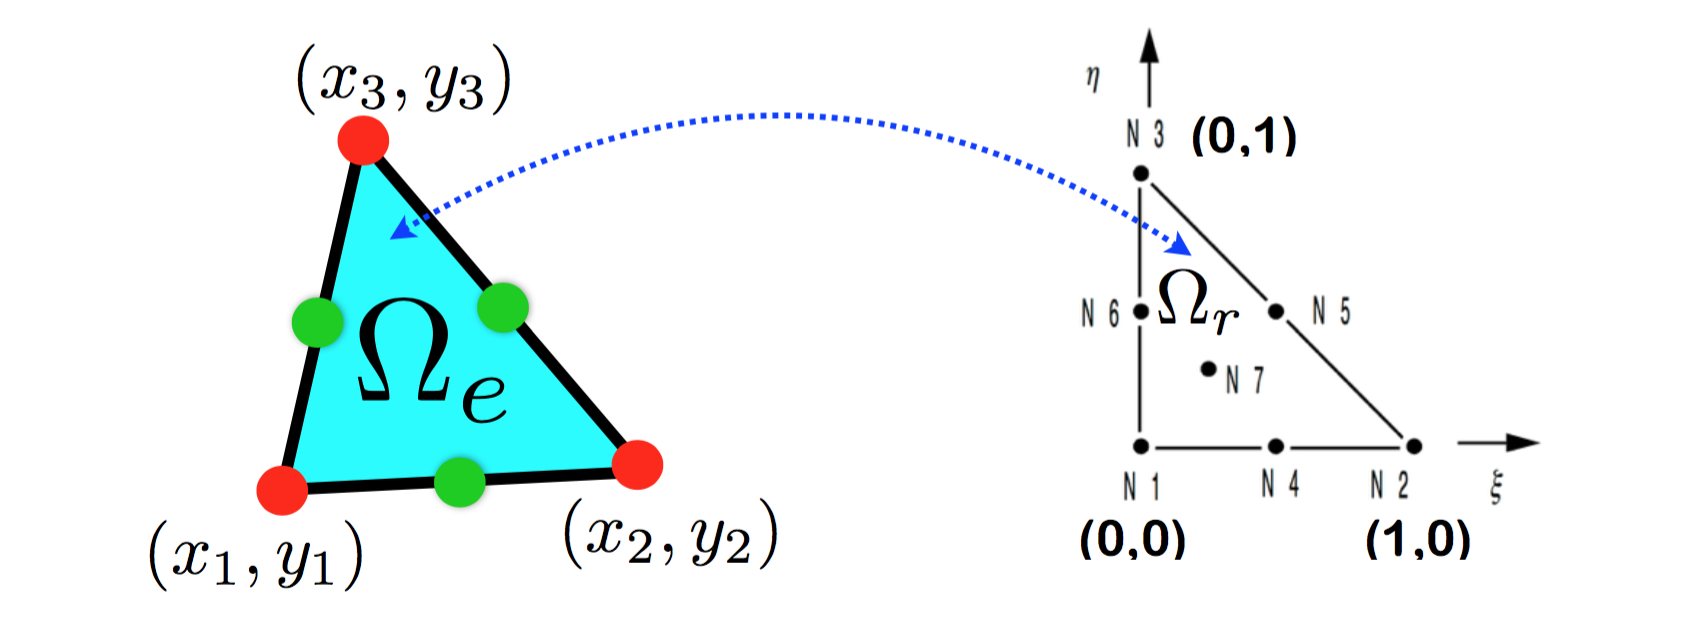
\includegraphics[width=0.7\textwidth]{../TeX_Files/Calculus/reference_element.png}
 \end{center}
 A given triangle $\mc{T}$ of vertices $(x_1,y_1)$, $(x_2,y_2)$ and $(x_3,y_3)$ is transformed into an isosceles rectangle triangle $\mc{T}_{ref}$. A point of coordinates $(x,y)$ in $\mc{T}$ is associated to a point $(\xi,\eta)$ in $\mc{T}_{ref}$. The transformation is then as follows:
 \begin{equation}
 f:\left\{
 \begin{array}{ccc}
 	\mc{T}_{ref} &\longrightarrow &\mc{T}\\
 	\begin{Bmatrix}
 		\xi\\\eta
 	\end{Bmatrix}
 	&\mapsto & 	\begin{Bmatrix}
 		x(\xi,\eta)\\
 		y(\xi,\eta)
 		 	\end{Bmatrix}
 \end{array}
 \right.	
 \end{equation}
This transformation relates the vertices as follows
\begin{align}
	f(0,0)&=(x_1,y_1)\\
	f(1,0)&=(x_2,y_2)\\
	f(0,1)&=(x_3,y_3)\\
\end{align} 
 

 \begin{itemize}
 	\item What is the expression of matrix $\{\bs{\Phi}(\xi,\eta)\}$ so that 
 \begin{equation}
 	\begin{Bmatrix}
 		x(\xi,\eta)\\
 		y(\xi,\eta)
 		 	\end{Bmatrix}=\begin{bmatrix}
 		 		x_1 & x_2 & x_3\\
 		 		y_1 & y_2 & y_3
 		 	\end{bmatrix}\{\bs{\Phi}(\xi,\eta)\}
 \end{equation}
 Compute the Jacobian Matrix $J$ of transformation $f$. $J$ is defined as 
 \begin{equation}
 	J=\begin{bmatrix}
 		\dfrac{\p x}{\p \xi} & \dfrac{\p x}{\p \eta}\\
 		\dfrac{\p y}{\p \xi} & \dfrac{\p y}{\p \eta}
 	\end{bmatrix}
 \end{equation} 
 \end{itemize}
  
\eexo

\solution{
\begin{equation}
	\{\bs{\Phi}(\xi,\eta)\}=\begin{Bmatrix}
		1-\eta-\xi \\ \xi \\ \eta
	\end{Bmatrix}
\end{equation}

 \begin{equation}
 	J=\begin{bmatrix}
 		-x_1+x_2 & -x_1+x_3\\
 		-y_1+y_2 & -y_1+y_3
 	\end{bmatrix}
 \end{equation} 


}
%% !TEX root = ../RAN_MFA.tex

\bexo
 What is the derivative of 
 \begin{equation}
 	f:x\mapsto {\sin(x)}{\cos^2(3x)}+\dfrac{\sin(x)}{\cos^2(3x)}+3\ln(2+\cos(x))+\tan(5x^2)
 	+\sin(x)\sin^2(3x)
 \end{equation}
 \eexo

\solution{
}
%% !TEX root = ../RAN_MFA.tex

\bexo
 Compute the Fourier coefficients of $x\mapsto \abs{x}$. They are defined by
 \begin{equation}
 	c_n=\dint{-\pi}{\pi} f(x)\cos(x) \,\d x 
 	\esp s_n=\dint{-\pi}{\pi} f(x)\sin(x) \,\d x 
 \end{equation}
\eexo

\solution{
}
%% !TEX root = ../RAN_MFA.tex

\bexo
 Gradient, Divergence and Curl operator in cartesian coordinates are given by 
$$\Gd f=\left|
\begin{array}{c}
\dfrac{\p f}{\p x}\\
\dfrac{\p f}{\p y}\\
\dfrac{\p f}{\p z}
\end{array}
\right. \esp
\Div \left|
\begin{array}{c}
f_x\\
f_y\\
f_z
\end{array}
\right.=\dfrac{\p f_x}{\p x}+
\dfrac{\p f_y}{\p y}
+\dfrac{\p f_z}{\p z}
\esp
\Rot \left|
\begin{array}{c}
f_x\\
f_y\\
f_z
\end{array}\right.=
\left|
\begin{array}{c}
\dfrac{\p f_z}{\p y}-\dfrac{\p f_y}{\p z}\\
\dfrac{\p f_x}{\p z}-\dfrac{\p f_z}{\p x}\\
\dfrac{\p f_y}{\p x}-\dfrac{\p f_x}{\p y}\\
\end{array}
\right.
$$

Polar coordinates are $\{r,\theta,Z\}$ and their link with cartesian coordinates are
$$ \left\{
\begin{array}{c}
x=r\,cos(\theta)\\
y=r\,sin(\theta)\\
z=Z
\end{array}
\right.$$
 
Spherical coordinates are $\{r,\theta,\phi\}$ and their link with cartesian coordinates are
$$ \left\{
\begin{array}{c}
x=r\,sin(\theta)\,cos(\phi)\\
y=r\,sin(\theta)\,sin(\phi)\\
z=r\,cos(\theta)
\end{array}
\right.$$ 
 

\begin{itemize}
\item What are the expression of the three differential operators in polar and spherical coordinates.
\end{itemize} 
\eexo

\solution{}
%% !TEX root = ../RAN_MFA.tex

\bexo
 The 1D wave equation in physical coordinates $(x,t)$ is 
 \begin{equation}
 	\dfrac{\p^2 p}{\p x^2}\dfrac{\p^2 p}{\p x^2}-\dfrac{\p^2 p}{\p t^2}=0
 \end{equation}
 Rewrite this equation in the coordinate system of characteristics $(X,Y)$ with
  \begin{equation}
  	X=x-ct \esp Y=x+ct.
  \end{equation}
 
\eexo

\solution{
}



%
%\chapter{Complex numbers}
%%
%\bexo
We are considering the superposition of an incident wave and a reflected plane wave
\be
p(x)=e^{-jkx}+Re^{jkx}
\ee 
What is the value of the physical pressure for
\begin{itemize}
\item $\omega=1$, $k=1$, $t=0$, $x=0$ and $R=1$
\item $\omega=\dfrac{\pi}{4}$, $k=1$, $t=1$, $x=0$ and $R=1$
\end{itemize}
\eexo

\solution{
The value of the pressure is:
\begin{itemize}
\item $p=2$
\item $p=\sqrt{2}$
\end{itemize}}
%\bexo 
\bi
\it Let consider a line $\mc{L}$ of equation $a x+b y+c=0$, with $a$, $b$ and $c$ three real numbers.  What is the complex equation of the line?
\it Let consider a circle of equation $(x-x_0)^2+(y-y_0)^2=R^2$, with $R$ the radius, and $x_0$ and $y_0$ two real numbers associated to the center of the circle. What is the complex equation of the circle ?\\
\it What is the inverse of $\mc{L}$?
\ei
\eexo

\solution{
\bi
\it
Let consider the expressions of real and imaginary parts of $z$ 
\be
x=\dfrac{z+\cj{z}}{2}\esp y=\dfrac{z-\cj{z}}{2j}
\ee
The equation of the line then becomes:
\be
\left(
\dfrac{a}{2}+\dfrac{b}{2j}
\right)z+\left(
\dfrac{a}{2}-\dfrac{b}{2j}
\right)\cj{z}+c=0
\ee
or
\be
\cj{\omega} z+\omega\cj{z}+c=0 \esp \omega=\left(
\dfrac{a}{2}+j\dfrac{b}{2}
\right)
\ee
\it
Let $z_0=x_0+jy_0$ be the complex number associated to the center of the circle. If one considers $z'=z-z_0$, the equation of the circle becomes
\be 
z'\cj{z'}=R^2
\ee
Hence the complex equation of the circle is:
\be 
z\cj{z}-z_0\cj{z}-\cj{z_0}z=R^2-\abs{z_0}^2.
\ee
\item Let $z$ be the affix of one element in the inverse of $\mc{L}$. Then $1/z$ is solution of the complex equation of the line:
\be
\dfrac{\cj{\omega}}{z}+\dfrac{\omega}{\cj{z}}+c=0
\ee
This equation becomes
\be
\cj{\omega}\cj{z}+{\omega}{z}+cz\cj{z}=0
\ee
We can identify a form close to a complex equation of a circle:
\be
z\cj{z}-z_0\cj{z}+\cj{z_0}{z}=0 \esp z_0=\dfrac{\cj{\omega}}{c}.
\ee
As the right hand side is null, the radius of the circle is $\abs{z_0}$:
\be
z\cj{z}-z_0\cj{z}+\cj{z_0}{z}=R^2-\abs{z_0}^2 \esp z_0=\dfrac{\cj{\omega}}{c}\esp 
R=\abs{z_0}.
\ee
\ei
}
%\bexo 

\bi
\it $f(t)=t\, e^{it}$
%\it $Z(\omega)=1+j\omega$
\ei
Plot the following parametric curves :
\bi
\it $(t,\re{f_1(t)})$, $(t,\im{f_1(t)})$, $(\re{f_1(t)},\im{f_1(t)})$
\ei


\eexo

\solution{
%\begin{figure}
The plots are
\bi
\it $(t,\re{f_1(t)})$, $(t,\im{f_1(t)})$, $(\re{f_1(t)},\im{f_1(t)})$\\
\includegraphics[height=50mm]{../TeX_Files/Complex_Numbers/complex_plots_1.eps}
\hfill
\includegraphics[height=50mm]{../TeX_Files/Complex_Numbers/complex_plots_2.eps}
\ei
%\end{figure}
}





%\bexo
The reflexion coefficient at an interface between two media (of reduced impedance $Z_1$ and $Z_2$) for a plane wave at normal incidence are given by the following formula
\begin{equation*}
R=\dfrac{Z_2-Z_1}{Z_2+Z_1}\esp 
T=\dfrac{2Z_2}{Z_2+Z_1}
\end{equation*}

Compute $R$ and $T$ in cartesian and polar form for 
\begin{equation}
Z_1=1\esp 
Z_2=i
\end{equation}
\eexo



\solution{
\begin{itemize}
\item ${R}=i$
\item ${T}=1+i$
\item $\abs{R}=1$ 
\item $\tr{arg}(R)=\dfrac{\pi}{2}$
\item $\abs{T}=\sqrt{2}$
\item $\tr{arg}(T)=\dfrac{\pi}{4}$
\end{itemize}
}
%\bexo 

What is the formal value (modulus, argument, real part, imaginary part) of $P=-e^{-jkx}$ for 
\begin{itemize}
\item $k=1+j[\ln(\pi)-ln(4)]$ and $x=\dfrac{\pi}{4}$
\end{itemize}



\eexo

\solution{
\more
}
%% !TEX root = ../RAN_MFA.tex

\bexo
 We are considering a monochromatic plane wave (circular frequency $\omega$ with a temporal dependance $e^{j\omega t}$) propagating in the 3D air. The complex representation of the pressure field is 
$$
p(x,t)=\hat{p}e^{j(\omega t-k_x x+k_y y +k_zz)},
$$
where $\{x,y,z\}$ are the cartesian coordinates and $\{k_x,k_y,k_z\}$ the components of the wave vector.\\

The parameter of the air are its density $\rho$ and celerity $c$. Euler's equation and the constitutive law in the time domain read:
$$ 
\rho \dfrac{\p v}{\p t}=-\Gd p \esp p=-\rho c^2 \Div u \esp v=\dfrac{\p u}{\p t}.
$$
 

\begin{itemize}
\item From Euler's equation, provide the expression of the complex amplitude of the velocity $\hat{\tb{v}}$
\item Find the dispersion relation: i.e. the relation between the wave number components, the circular frequency and the properties of the medium 
\end{itemize} 
\eexo

\solution{
\begin{itemize}
\item $\hat{\tb{v}}=\hat{p}\left\{
\begin{array}{c}
k_x\\
k_y\\
k_z
\end{array}
\right.$
\item $k_x^2+k_y^2+k_z^2=\dfrac{\omega^2}{c^2}$
\end{itemize} 
}
%\bexo
Let consider polynomial  
\begin{equation}
	P(X)=X^3+(1+j)X^2+(-6+j)X-6j \esp j=\sqrt{1}.
\end{equation}
\begin{itemize}
	\item Show that $-j$ is a root of $P$.
	\item Find the two other roots.
\end{itemize} 
 
\eexo
\solution{
\begin{align}
	P(j)&=j-(1+j)-j(-6+j)-6j=j-1-j+6j+1-6j=0
\end{align}




$-j$ is then one root of the polynomial. It is then possible to factorize $P$ by $(X+j)$. This can be done by two means. \\

The first one is euclidian division
\begin{equation}
	\begin{array}{rrrrrrrrrr|l}
	        &{X^3}&{+}&{(1+j)}&{X^2}&{+}&{(-6+j)}&{X}&{-}&{6j}&{X+j}\\	\cline{11-11} 
\od{-}&	     {X^3}&{+}&{j}    &{X^2}&   &        &   &   &    &{X^2+X-6}\\ \cline{1-10} 
      &           &   &       &{X^2}&{+}&{(-6+j)}&{X}&{-}&{6j}\\
\od{-}&           &   &       &{X^2}&{+}&{j}&{X}&&\\    \cline{5-10} 
      &           &   &       &     &{}&{-6}&{X}&-&6j\\  
 \od{-}           &           &   &       &     &{}&{-6}&{X}&-&6j\\ \cline{7-10} 
       &           &   &       &     &{}&{}&{}&&\tb{0}\\           
	\end{array}
\end{equation}


The second method is the identification 

\begin{align}
	X^3+(1+j)X^2+(-6+j)X-6j&=(X+j)(aX^2+bX+c)\\
	&=aX^3+(b+ja)X^2+(c+bj)X+cj
\end{align}
By identification of the coefficients in $X^3$:
\begin{equation}
	a=1.
\end{equation}
By identification of the coefficients in $X^2$:
\begin{equation}
	b+ja=1+j \so b=1.
\end{equation}
By identification of the coefficients in $X$:
\begin{equation}
	c+bj=-6+j \so c=-6.
\end{equation}
We can check that this value of $c$ is ok and leads to an identification of the term of zero order. 
\begin{equation}
	c+bj=-6+j \so c=-6.
\end{equation}

The two other roots of out polynomial are the one of $X^2+X-6$. Once more, two methods to find the result. \\

The first one is the classical one
\begin{equation}
	\Delta=1^2+4\times 6=25=5^2
\end{equation}

The two roots are then
\begin{equation}
	\dfrac{-1\pm\sqrt{\Delta}}{2}\so X=2 \tr{ and } X=-3.
\end{equation}

The second method corresponds to the formula
\begin{equation}
	(X-x_1)(X-x_2)=X^2-(x_1+x_2)X+x_1x_2
\end{equation}
Hence $x_1+x_2=-1$ and $x_1x_2=-6$. The two roots are then $x_1=2$ and $x_2=-3$.

}
%\bexo 

\bi
\it $f(t)=t\, e^{it}$
%\it $Z(\omega)=1+j\omega$
\ei
Plot the following parametric curves :
\bi
\it $(t,\re{f_1(t)})$, $(t,\im{f_1(t)})$, $(\re{f_1(t)},\im{f_1(t)})$
\ei


\eexo

\solution{
%\begin{figure}
The plots are
\bi
\it $(t,\re{f_1(t)})$, $(t,\im{f_1(t)})$, $(\re{f_1(t)},\im{f_1(t)})$\\
\includegraphics[height=50mm]{FIG/complex_plots_1.eps}
\hfill
\includegraphics[height=50mm]{FIG/complex_plots_2.eps}
\ei
%\end{figure}
}
%\bexo
Let consider two harmonic (at circular frequency $\omega$) fields $p(t)$ and $v(t)$. In complex representation, with a positive time convention $\e^{+j\omega t}$, their complex amplitudes are respectively denoted by $\hat{p}$ and $\hat{v}$.\\

The energy flow $W(t)$ at time $t$ is given by 
\begin{equation} 
W(t)=p(t)v(t).
\end{equation}

The average operator for any periodic function $P(t)$ of period $T$ is given by:
\begin{equation}
<P>=\dfrac{1}{T} \ds{\int_0^{T}} P(t) \d t.
\end{equation}

\begin{itemize}
\item What is the value of $<v>$ ?
\item What is the value of $<W>$ ? 
\end{itemize}\eexo


\solution{

$<v>=0$ trivially as in this case $T=2\pi/\omega$
\begin{align}
	<v>=\dfrac{1}{T} \ds{\int_0^{T}} \re{\hat{v}e^{j\omega t}} \d t&=\dfrac{1}{T} \re{\ds{\int_0^{T}} \hat{v}e^{j\omega t} \d t}\\
		&=\dfrac{1}{T} \re{\hat{v} \left[\dfrac{e^{j\omega t}}{j\omega} \right]_0^T}=0
\end{align}

Concerning $W$
\begin{align}
	<W>&=\dfrac{1}{T} \ds{\int_0^{T}} \re{\hat{p}e^{j\omega t}}\re{\hat{v}e^{j\omega t}} \d t\\
	   &=\dfrac{1}{T} \ds{\int_0^{T}} \left[
	   \dfrac{\hat{p}e^{j\omega t}+\hat{p}\st e^{-j\omega t} }{2}
	   \dfrac{\hat{v}e^{j\omega t}+\hat{v}\st e^{-j\omega t} }{2}
	   \right] \d t\\
	   	    &=\dfrac{1}{4T} 
	   	    \ds{\int_0^{T}} \left[
	   \hat{p}\hat{v}e^{2j\omega t}+\hat{p}\hat{v} \st
	   +\hat{p}\st\hat{v}+\hat{v}\st\hat{p}\st e^{-2j\omega t}
	   \right] \d t
\end{align}
The two oscillating terms are zero averaged. The other are constants Hence 
\begin{align}
	<W>&=
	    \dfrac{1}{4T} \ds{\int_0^{T}} \left[
	   \hat{p}\hat{v}\st+\hat{p}\st\hat{v}  \right] \d t =\dfrac{1}{4T}  \left[
	   \hat{p}\hat{v}\st+\hat{p}\st\hat{v}  \right] T\\
	   &=\dfrac{1}{2}\re{\hat{p}\hat{v}\st}.
\end{align}

}



%
%
%
%
%\chapter{Ordinary Differential Equations}
%
%\section{First order equations}



%\bexo
What is the solution of  
\begin{equation}
	f''(x)-f'(x)-12f(x)-12=0,
\end{equation}
with 
\begin{equation}
	f(0)=5,\, f'(0)=17.
\end{equation}

\eexo
\solution{
The solution of this equation is the sum of a particular solution which do not satisfy the initial conditions and a general one associated to the homogeneous problem \ie{without forcing}.
The particular solution is 
\begin{equation}
	f_p(x)=-1.
\end{equation}
The general solution is associated to 
\begin{equation}
	f''(x)-f'(x)-12f(x)=0.
\end{equation}
The characteristic polynomial is 
\begin{equation}
	p^2-p-12=0.
\end{equation}
The roots are $-3$ and $4$.\\
We are then looking for a function of the form
\begin{equation}
	f(x)=Ae^{-3x}+Be^{4x}-1.
\end{equation}
With the initial conditions
\begin{equation}
	f(0)=A+B-1=5\esp f'(0)=-3A+4B=17.
\end{equation}
Hence: 
\begin{equation}
	A=1\esp B=5\so f(x)=e^{-3x}+5e^{4x}-1.
\end{equation}
}

%\bexo
What is the solution of  
\begin{equation}
-f'(x)+f(x)=1+x,
\end{equation}
with 
\begin{equation}
	f(0)=2,\, f'(0)=1.
\end{equation}

\eexo
\solution{
The solution of this equation is the sum of a particular solution which do not satisfy the initial conditions and a general one associated to the homogeneous problem \ie{without forcing}.
The particular solution is sought as a first order polynomial 
\begin{equation}
	f_p(x)=ax+b.
\end{equation}
Hence, the necessary conditions on $a$ and $b$ are:
 \begin{equation}
	-f_p'(x)+f_p(x)=-a+ax+b=1+x.
\end{equation}
By identification 
\begin{equation}
	a=1 \and b=2. 
\end{equation}
Hence 
\begin{equation}
	f_p(x)=x+2
\end{equation}
This function satisfies the initial conditions. We have our solution and there is no need of a general solution of the homogeneous equation ! 
}

%\bexo
What is the solution of  
\begin{equation}
	m\ddot{x}(t)+c\ddot{x}(t)+kx(t)=F\cos(\omega t),
\end{equation}
with 
\begin{equation}
	x(0)=0,\, \dot{x}(0)=0.
\end{equation}

\eexo
\solution{


\begin{equation}
	\ddot{x}(t)+\mu\ddot{x}(t)+\omega_0^2 x(t)=F'\cos(\omega t)\esp F'=\dfrac{F}{m}\esp \mu=\dfrac{c}{m}.
\end{equation}


The particular solution 
\begin{equation}
	x_p(t)=A\cos(\omega t)+B\sin(\omega t).
\end{equation}


\begin{equation}
	(\omega^2_0-\omega^2)(A\cos(\omega t)+B\sin(\omega t))+\omega \mu (-A\sin(\omega t)+B\cos(\omega t))=F'\cos(\omega t).
\end{equation}


\begin{equation}
	\left[
		\begin{array}{cc}
		{\omega^2_0-\omega^2m}&{\omega \mu}\\
		{-\omega \mu}&{\omega^2_0-\omega^2}
	\end{array}
	\right]\left\{
	\begin{array}{c}
		{A}\\
		{B}
	\end{array}
	\right\}=\left\{
	\begin{array}{c}
		{F'}\\
		{0}
	\end{array}
	\right\}
\end{equation}

A necessary condition 

\begin{equation}
	(\omega^2_0-\omega^2)^2+\omega^2\mu^2 >0
\end{equation}

\begin{equation}
	A=\dfrac{F'(\omega^2_0-\omega^2 )}{(\omega^2_0-\omega^2)^2+\omega^2\mu^2} \esp B=\dfrac{F'\omega \mu}{(\omega^2_0-\omega^2)^2+\omega^2\mu^2} 
\end{equation}

\begin{equation}
	x_p(t)=\dfrac{F'}{\sqrt{(\omega^2_0-\omega^2)^2+\omega^2\mu^2}}\left(
	\cos(\phi)
	\cos(\omega t)+\sin(\phi) \sin(\omega t)
	\right)
\end{equation}
with
\begin{equation}
	\cos(\phi)=\dfrac{\omega^2_0-\omega^2}{\sqrt{(\omega^2_0-\omega^2)^2+\omega^2\mu^2}} \esp
	\sin(\phi)=\dfrac{\omega \mu}{\sqrt{(\omega^2_0-\omega^2)^2+\omega^2\mu^2}}
\end{equation}

\begin{equation}
	x_p(t)=\dfrac{F'}{\sqrt{(k-\omega^2m)^2+\omega^2c^2}}
	\cos(\omega t-\phi)
\end{equation}



\begin{equation}
	\ddot{x}(t)+\mu\ddot{x}(t)+\omega_0^2 x(t)=0, x(t)=exp(-\alpha t)
\end{equation}



}

%\bexo
We are considering the harmonic damped oscillator\footnote{oscillator harmonique amorti} of a mass $m$ linked to a rigid support by a spring\footnote{ressort} $k$. An external force $f(t)$ can be applied to this dynamical system. Hence the displacement $x(t)$ of the mass is governed by
\begin{equation}
	m\ddot{x}(t)+kx(t)=f(t).
\end{equation}
The numerical values of the parameters are 
\begin{equation}
	m=1 \esp k=1.
\end{equation}
At time $t=0$ , the initial condition of the system are
\begin{equation}
	x(0)=0\esp \dot{x}(0)=1.
\end{equation}
at time $t=1$, a constant force $f=-1$ is applied to the mass. 

\begin{itemize}
	\item What is the expression of the displacement $x(t)$ ?
\end{itemize}



%\begin{figure}[h]
%\begin{center}
%\begin{tikzpicture}
%\path (-40mm,0);
%\node[mass] at (2.4,0) {};
%\draw[spring] (0,0.5) -- (1.65,0.5); 
%\draw [damper] (0,-0.5) -- (1.65,-0.5);
%% Rigid body
%\draw[thick] (0,-1.5) -- (0,1.2);
%\fill [pattern = north east lines] (-0.3,-1.5) rectangle (0,1.2);
%\node[text width=5cm] at (3.2,0.1) {$k$};
%\node[text width=5cm] at (3.2,-1) {$c$};
%\node[text width=5cm] at (4.6,1) {$m$};
%\node[text width=5cm] at (4.6,-1) {$x(t)$};
%% Force under the mass
%\draw [thick] (2.2,-1.4) -- (2.2,-1.2);
%\draw [thick, ->] (2.2,-1.4) -- (2.7,-1.4);
%\node[text width=5cm] at (4.5,-1.7) {$M f(t)$};
%\end{tikzpicture}
%\end{center}
%\end{figure}



\eexo
\solution{


\begin{equation}
	\ddot{x}(t)+\mu\ddot{x}(t)+\omega_0^2 x(t)=F'\cos(\omega t)\esp F'=\dfrac{F}{m}\esp \mu=\dfrac{c}{m}.
\end{equation}


The particular solution 
\begin{equation}
	x_p(t)=A\cos(\omega t)+B\sin(\omega t).
\end{equation}


\begin{equation}
	(\omega^2_0-\omega^2)(A\cos(\omega t)+B\sin(\omega t))+\omega \mu (-A\sin(\omega t)+B\cos(\omega t))=F'\cos(\omega t).
\end{equation}


\begin{equation}
	\left[
		\begin{array}{cc}
		{\omega^2_0-\omega^2m}&{\omega \mu}\\
		{-\omega \mu}&{\omega^2_0-\omega^2}
	\end{array}
	\right]\left\{
	\begin{array}{c}
		{A}\\
		{B}
	\end{array}
	\right\}=\left\{
	\begin{array}{c}
		{F'}\\
		{0}
	\end{array}
	\right\}
\end{equation}

A necessary condition 

\begin{equation}
	(\omega^2_0-\omega^2)^2+\omega^2\mu^2 >0
\end{equation}

\begin{equation}
	A=\dfrac{F'(\omega^2_0-\omega^2 )}{(\omega^2_0-\omega^2)^2+\omega^2\mu^2} \esp B=\dfrac{F'\omega \mu}{(\omega^2_0-\omega^2)^2+\omega^2\mu^2} 
\end{equation}

\begin{equation}
	x_p(t)=\dfrac{F'}{\sqrt{(\omega^2_0-\omega^2)^2+\omega^2\mu^2}}\left(
	\cos(\phi)
	\cos(\omega t)+\sin(\phi) \sin(\omega t)
	\right)
\end{equation}
with
\begin{equation}
	\cos(\phi)=\dfrac{\omega^2_0-\omega^2}{\sqrt{(\omega^2_0-\omega^2)^2+\omega^2\mu^2}} \esp
	\sin(\phi)=\dfrac{\omega \mu}{\sqrt{(\omega^2_0-\omega^2)^2+\omega^2\mu^2}}
\end{equation}

\begin{equation}
	x_p(t)=\dfrac{F'}{\sqrt{(k-\omega^2m)^2+\omega^2c^2}}
	\cos(\omega t-\phi)
\end{equation}



\begin{equation}
	\ddot{x}(t)+\mu\ddot{x}(t)+\omega_0^2 x(t)=0, x(t)=exp(-\alpha t)
\end{equation}



}

%\bexo
What is the solution of  
\begin{equation}
	m\ddot{x}(t)+c\ddot{x}(t)+kx(t)=F\cos(\omega t),
\end{equation}
with 
\begin{equation}
	x(0)=0,\, \dot{x}(0)=0.
\end{equation}

\eexo
\solution{


\begin{equation}
	\ddot{x}(t)+\mu\ddot{x}(t)+\omega_0^2 x(t)=F'\cos(\omega t)\esp F'=\dfrac{F}{m}\esp \mu=\dfrac{c}{m}.
\end{equation}


The particular solution 
\begin{equation}
	x_p(t)=A\cos(\omega t)+B\sin(\omega t).
\end{equation}


\begin{equation}
	(\omega^2_0-\omega^2)(A\cos(\omega t)+B\sin(\omega t))+\omega \mu (-A\sin(\omega t)+B\cos(\omega t))=F'\cos(\omega t).
\end{equation}


\begin{equation}
	\left[
		\begin{array}{cc}
		{\omega^2_0-\omega^2m}&{\omega \mu}\\
		{-\omega \mu}&{\omega^2_0-\omega^2}
	\end{array}
	\right]\left\{
	\begin{array}{c}
		{A}\\
		{B}
	\end{array}
	\right\}=\left\{
	\begin{array}{c}
		{F'}\\
		{0}
	\end{array}
	\right\}
\end{equation}

A necessary condition 

\begin{equation}
	(\omega^2_0-\omega^2)^2+\omega^2\mu^2 >0
\end{equation}

\begin{equation}
	A=\dfrac{F'(\omega^2_0-\omega^2 )}{(\omega^2_0-\omega^2)^2+\omega^2\mu^2} \esp B=\dfrac{F'\omega \mu}{(\omega^2_0-\omega^2)^2+\omega^2\mu^2} 
\end{equation}

\begin{equation}
	x_p(t)=\dfrac{F'}{\sqrt{(\omega^2_0-\omega^2)^2+\omega^2\mu^2}}\left(
	\cos(\phi)
	\cos(\omega t)+\sin(\phi) \sin(\omega t)
	\right)
\end{equation}
with
\begin{equation}
	\cos(\phi)=\dfrac{\omega^2_0-\omega^2}{\sqrt{(\omega^2_0-\omega^2)^2+\omega^2\mu^2}} \esp
	\sin(\phi)=\dfrac{\omega \mu}{\sqrt{(\omega^2_0-\omega^2)^2+\omega^2\mu^2}}
\end{equation}

\begin{equation}
	x_p(t)=\dfrac{F'}{\sqrt{(k-\omega^2m)^2+\omega^2c^2}}
	\cos(\omega t-\phi)
\end{equation}



\begin{equation}
	\ddot{x}(t)+\mu\ddot{x}(t)+\omega_0^2 x(t)=0, x(t)=exp(-\alpha t)
\end{equation}



}




\end{document}
\end

